\section{Die Layout-Manager}

In diesem Kapitel werden die Layout- oder Gemeometrie-Manager von Tkinter behandelt.
Grunds�tzlich stehen drei verschiedene Layout-Manager zur Verf�gung:

\begin{itemize}
    \item Pack
    \item Grid
    \item Place
\end{itemize}

Layout-Manager dienen in erster Linie dazu, Widgets in einem Wurzel-Element zu regestrieren,
anzuordnen und darzustellen. Besonders die Anordnung durch Angabe von Position und Gr��e eines Widgets
wird durch die Layout-Manager stark vereinfacht.

Einem Wurzel-Element sollte immer nur ein Layout-Manager angeh�ngt werden.

\subsection{Pack}

Der Pack-Manager ist der am einfachsten zu verwendende Layout-Manager.
Hier werden Widgets in Zeilen oder Spalten (vertikal oder horizontal) 'gepackt' und durch Optionen wie
\lstinline$fill$ oder \lstinline$expand$ gesteuert.

Im Vergleich zu dem sehr �hnlichen Grid-Manager ist der Pack-Manager etwas eingeschr�nkt,
aber in einigen wenigen Situationen sinnvoller zu nutzen. Speziell wenn einfache
Widgets �bereinander oder nebeneinander angeordnet werden, oder Inhalte eines Widgets das gesamte
�bergeordnete Widget ausf�llen sollen wird der Pack-Manager bevorzugt.

Das folgende Beispiel soll die Effekte des Pack-Managers verdeutlichen:

\lstinputlisting[language=Python]{chapters/userInterface/src/GUI_PackExample.py}
\label{gui:gui_packexample}

\begin{figure}[ht]
	\centering
	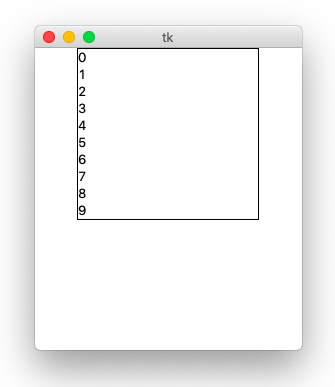
\includegraphics[width=0.5\textwidth]{images/PackManagerGUI_II.png}
	\caption{Listbox Widget mit einem Pack-Manager angeordnet}
	\label{fig:PackManagerGUI_I}
\end{figure}

Standardm��ig wird die Gr��e der Listbox so gew�hlt, dass Zehn Elemente angezeigt
werden k�nnen. Im obigen Quelltext werden der Listbox allerdings doppelt so viele Elemente
�bergeben. Versucht der User nun das Wurzel-Element, sprich das Fenster, zu verg��ern
um alle Elemente anzuzeigen, erzeugt Tkinter rund um das Listbox-Widget einen Abstand zum Fenster.
Um das Widget der gesamten zur Verf�gung stehenden Fl�che anzupassen, m�ssen die
Optionen \lstinline$fill$ und \lstinline$expand$ des Pack-Managers angesprochen werden.

\lstinputlisting[language=Python]{chapters/userInterface/src/GUI_PackExampleII.py}
\label{gui:gui_packexample}

\begin{figure}[ht]
	\centering
	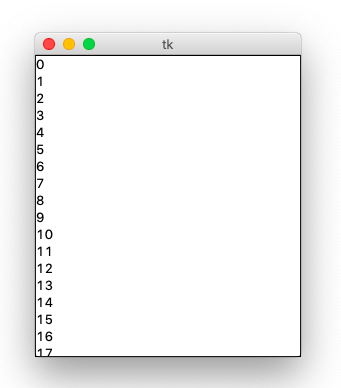
\includegraphics[width=0.5\textwidth]{images/PackManagerGUI_I.png}
	\caption{Listbox Widget mit einem Pack-Manager angeordnet unter Angabe von fill und expand}
	\label{fig:PackManagerGUI_II}
\end{figure}

Die \lstinline$fill$-Option teilt dem Pack-Manager mit, dass der gesamte zur Verf�gung
stehende Raum durch das Widget ausgef�llt werden soll. Der dahinter stehende Wert
regelt wie der Raum gef�llt wird. \lstinline$BOTH$ bedeutet, dass das Widget
sowohl horizontal als auch vertikal expandieren soll.
Alternativ kann der Raum mit der Angabe \lstinline$X$ nur horizontal und mit der Angabe
\lstinline$Y$ nur vertikal ausgef�llt werden.

Dar�ber hinaus k�nnen Widgets mithilfe der Layout-Manager angeordnet werden.
Der Pack-Manager richtet Widgets, ohne weitere Angaben von Optionen, vertikal, sprich in Spalten aus.

\lstinputlisting[language=Python]{chapters/userInterface/src/GUI_PackExampleIII.py}
\label{gui:gui_packexampleIII}

\begin{figure}[ht]
	\centering
	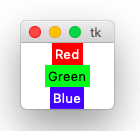
\includegraphics[width=0.3\textwidth]{images/PackManagerGUI_III.png}
	\caption{Mit Pack-Manager vertikal angeordnete Label-Widgets}
	\label{fig:PackManagerGUI_III}
\end{figure}

�ber die Option \lstinline$fill=X$ (horizontal) kann die Breite der Labels dem Eltern-Element angepasst werden.

\lstinputlisting[language=Python]{chapters/userInterface/src/GUI_PackExampleIV.py}
\label{gui:gui_packexampleIV}

\begin{figure}[ht]
	\centering
	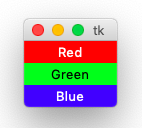
\includegraphics[width=0.3\textwidth]{images/PackManagerGUI_IV.png}
	\caption{Mit Pack-Manager vertikal angeordnete Label-Widgets unter Angabe von fill}
	\label{fig:PackManagerGUI_IV}
\end{figure}

Neben der vertikalen Ausrichtung der labels ist auch eine horizontale m�glich, dazu steht
die \lstinline$side$-Option zur Verf�gung. Mit \lstinline$side=LEFT$ werden die
Widgets von links beginnend angeordnet. Weitere Paramter sind \lstinline$side=TOP$ (default),
\lstinline$side=BOTTOM$ und \lstinline$side=RIGHT$.

\subsection{Grid}

Der Grid-Manager ist der am flexibelsten einzusetzende Layout-Manager von Tkinter.
Besonders komfortabel ist der Einsatz bei dem Gestalten von Dialogfeldern. Die Handhabung
ist denkbar einfach. Das folgende Schaubild erl�utert die Aufteilung eines Gitterrasters:

\begin{figure}[ht]
	\centering
	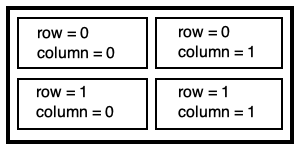
\includegraphics[width=0.4\textwidth]{images/GridManagerGUI.png}
	\caption{Gitterraster mit zwei Spalten und Reihen}
	\label{fig:GridManagerGUI}
\end{figure}

Nach dem Erzeugen eines Widget-Elementes kann es �ber den Methoden-
Aufruf des Grid-Managers, unter Angabe von Zeilen und Spalten ausgerichtet
werden. Dabei muss weder H�he noch Breite der entsprechenden Zelle angegeben werden, der
Grid-Manager passt diese dem Content des Widgets an.

\lstinputlisting[language=Python]{chapters/userInterface/src/GUI_GridExampleI.py}
\label{gui:gui_gridexampleI}

\begin{figure}[ht]
	\centering
	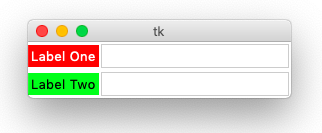
\includegraphics[width=0.5\textwidth]{images/GridManagerGUI_I.png}
	\caption{Mit Grid-Manager angeordnete Label- und Input-Widgets}
	\label{fig:GridManagerGUI_I}
\end{figure}

Leere Spalten und Zeilen werden von dem Layout-Manager ignoriert, das Ergebnis w�re
das selbe wenn die Angabe anstelle von \lstinline$grid(row=0)$ und \lstinline$grid(row=1)$,
\lstinline$grid(row=5)$ und \lstinline$grid(row=10)$ lauten w�rde.

Der Inhalt der Zellen wird ohne weiter Angaben mittig angeordnet, was �ber die \lstinline$sticky$-Option
ge�ndert werden kann. Im Gegensatz zu der \lstinline$side$-Option des Pack-Managers,
nimmt \lstinline$sticky$ Himmelsrichtungen, also N, E, S und W als Angabe entgegen.
Mit \lstinline$Label(...).grid(row=0, sticky=W)$
beginnt der Text des Label-Widgets am linken Zellenrand (Westen). Auch Kombinationen wie Beispielsweise
'unten links' (\lstinline$sticky=W+S$) sind m�glich.

\subsection{Place}

Der dritte Layout-Manager von Tkinter ist der Place-Manager. Hier kann die Position und Gr��e eines
 Fensters explizit festgelegt werden, entweder absolut oder relativ zu einem anderen Fenster.
In der Regel werden Pack- oder Grid-Manager f�r die Gestaltung herk�mmlicher Dialog- und Fensteroberfl�chen
verwendet, in einigen wenigen F�llen ist jedoch der Place-Manager die bessere Wahl.
Beispielswei�e bei der Anordnung von Steuerelementen in Pop-Up Dialogen kommt der Place-Manager zum Einsatz.

Der Zugriff erfolgt wie bei ben vorherigen Layout-Managern �ber den Methodenaufruf unter Angabe
von X und Y - Koordinaten. Alternativ k�nnen mit der \lstinline$anchor$-Option �hnlich
der \lstinline$side$-Option des Pack-Managers, die Widgets �ber Kompass-Richtungen
ausgerichtet werden. Default ist NW (obere rechte Ecke des Eltern-Elements).

\subsection{Zusammenfassung}

Zusammenfassend kann gesagt werden:

\begin{itemize}
    \item Der Pack-Manger organisiert Widget-Elemente in Blocks, bevor diese im Eltern-Element platziert werden.
    \item Der Grid-Manger platziert Widget-Elemente in einer Tabellenartigen Struktur im Elter-Element.
    \item Der Place-Manager platziert Widget-Elemente in spezifischer Position im Eltern-Element.
\end{itemize}
